All the main PAH features features, including the 6.2, 7.7, 8.6 and 11.3 $\mu$m bands, are clearly visible in the final processed spectra (see Figures \ref{PAHFITplots}) from all the regions except the nucleus (The spectrum of the nucleus is discussed in Section 4.3). They also show atomic line emissions such as [Ar~{\sc ii}], [Ar~{\sc iii}], [S~{\sc iii}], [S~{\sc iv}], [Ne~{\sc ii}], [Ne~{\sc iii}] and molecular $H_{2}$ emission at 12.3 $\mu$m. Some of the spectra display a contribution to the continuum from starlight emission.

Dust continuum emission from the Regions 3 and 9 is very low compared to other spectra and they also show some negative flux values in the shorter wavelengths which can be due to instrumental errors. It was observed that the spectrum from the NGC 206 is very noisy, therefore that spectrum was removed from our analysis. 


\subsection{ISOCAM versus IRS }


As mentioned in the Introduction, based on ISOCAM observations \citet{1998Cesarsky} reported a suppression of the common 6 to 8 $\mu$m features and an enhancement of a broad 11.3 and 12.7 $\mu$m features in four regions of M31. In addition, \citet{Pagani_1999} confirmed that the star-forming ring in M31 shows very weak PAH emission in the 6 to 8 $\mu$m region. 
However, the IRS spectra presented here do not show such unusual behaviour (Figure \ref{PAHFITplots}). Indeed, except for the nucleus, all regions show a normal mid-IR spectrum similar to other nearby starforming galaxies. Therefore, we obtained newly-processed ISOCAM spectra from three regions in our IRS sample (see Section 2.4) and compare them with the corresponding IRS spectra (Figure \ref{ISOnIRS}). 

	The spectra from both instruments look almost the same. Although the relative intensity of the features in the IRS and ISOCAM spectra are differ in detail, the shapes of the spectra are almost identical. Except for the nucleus, there is no depletion in 6 to 8 $\mu$m features as described in \citet{1998Cesarsky}. 
	
	Until 2005, ISOCAM data were not properly background subtracted and they were contaminated with zodiacal emission and stray light. Therefore, differential spectra between regions of relatively strong and weak emission have been used to overcome this problem (more details about the differential spectra can be found in \citealt{1998Cesarsky}). In 2005, the ISOCAM data were reprocessed  and corrected for the zodiacal emission \citep{Boulanger_F_2005}. For the remainder of this paper the reprocessed ISOCAM data are referred to as ISO2005 and earlier data as ISO1998. It is clear that the spectra obtained from these newly processed ISOCAM data do not agree with the previous differential spectra, especially for the bulge and the nucleus. Indeed, the differential spectrum shows a broad emission around the 11.3 micron feature not visible in Figure \ref{ISOnIRS} (top). Also, the differential spectrum towards the bulge does not show any emission in the 6 to 8 $\mu$m region unlike the newly processed data (Figure \ref{ISOnIRS} middle).

	By examining the spectra obtained from other regions (Figure 8 $\&$ 9) which were observed by IRS instrument, it can be argued that the IRS results do not support the results based on ISO1998 data.


\begin{figure}
\centering
%\begin{center}
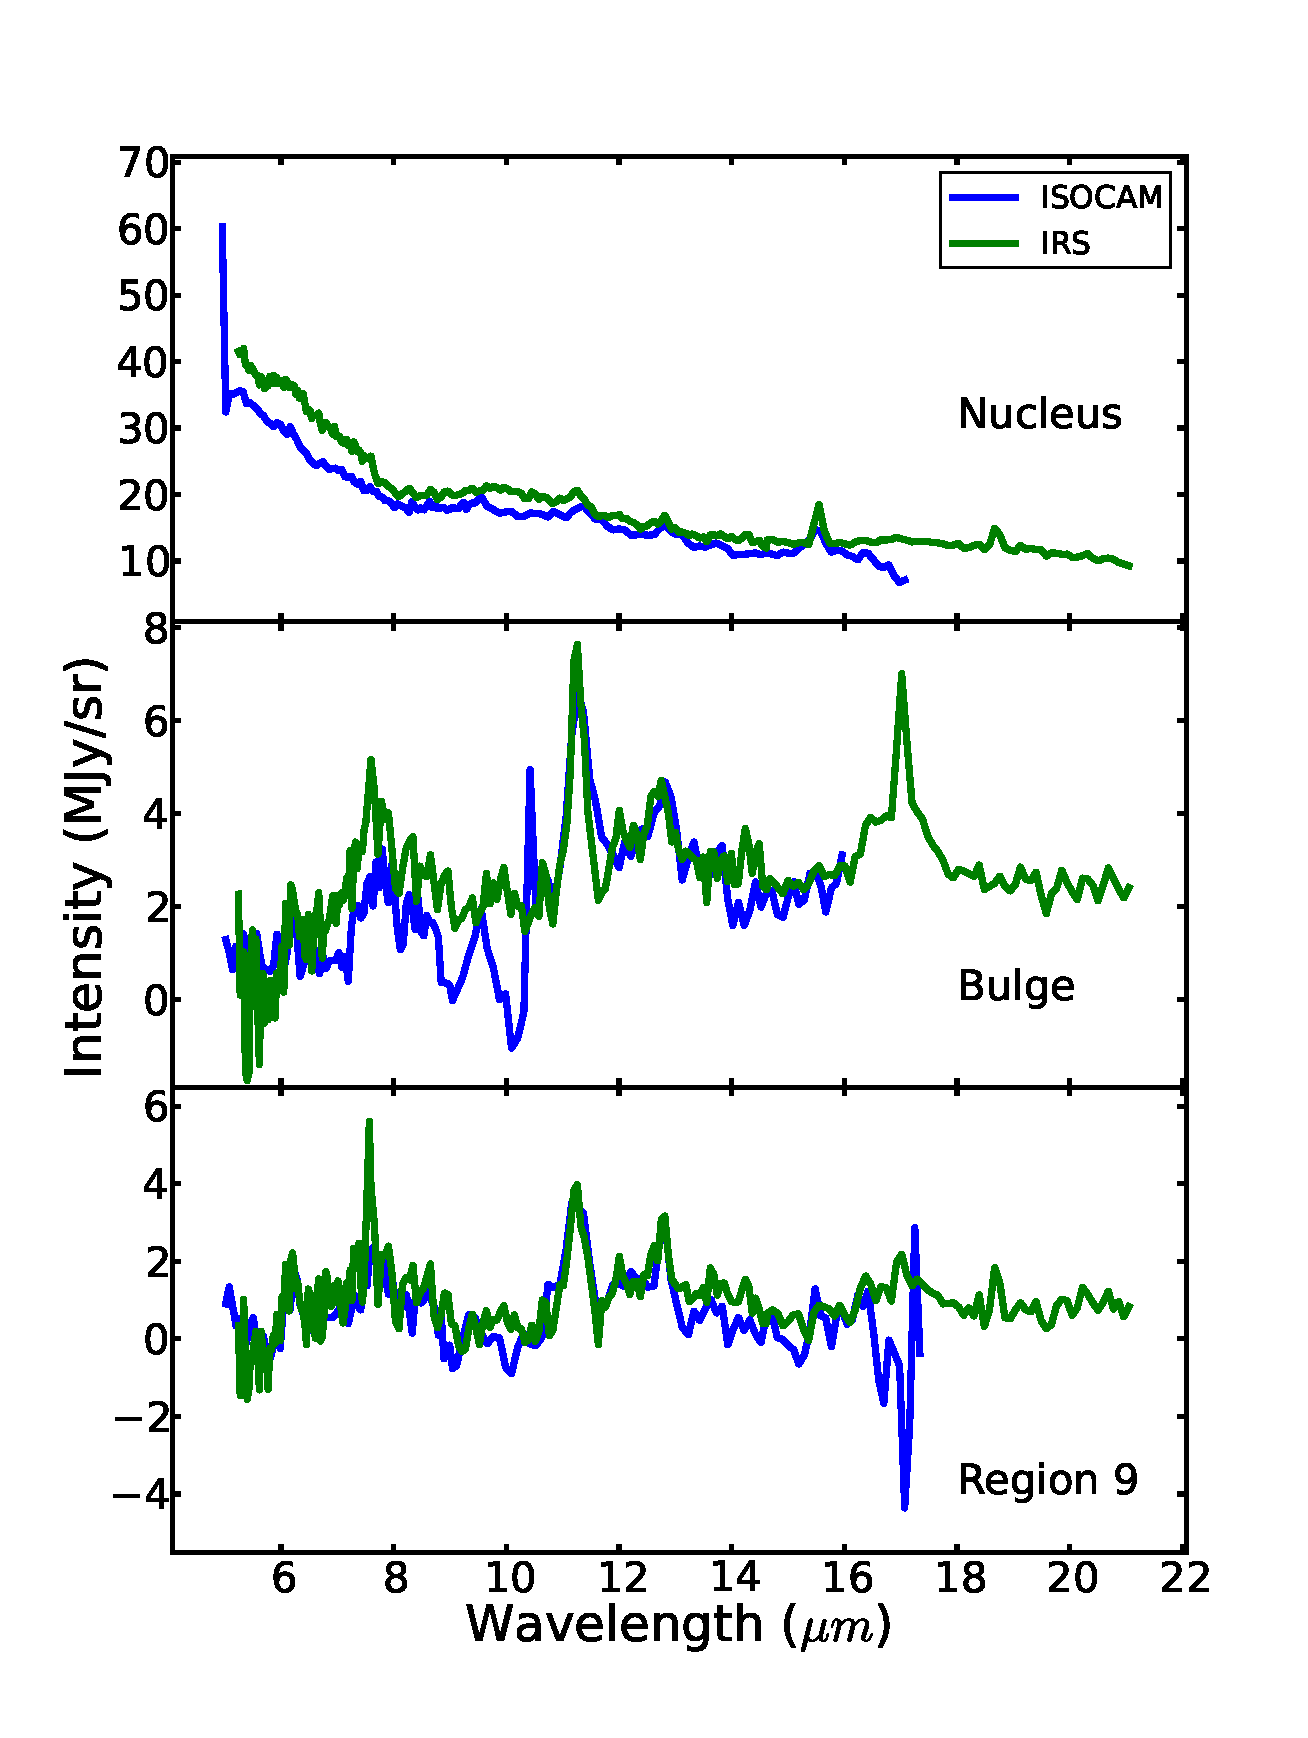
\includegraphics[scale=0.35]{./ISOvsIRS.eps}
\caption{ Comparison of the IRS and the newly processed ISOCAM spectra for the Nucleus (top), Bulge (middle) and Region 9 (bottom) in M31.}
%\end{center}
\label{ISOnIRS}
\end{figure}


\subsection{PAHFIT}

The PAH features in the IRS spectra are often blended with neighbouring aromatic features and atomic lines. Therefore measuring the strength of PAH features is difficult. To achieve this task a tool called PAHFIT, introduced by \citet{Smith:2007lr}, was used. PAHFIT is an IDL  based tool designed for decomposing {\em Spitzer} IRS spectra of PAH emission sources and is capable of identifying PAH features among other blended features. It also takes silicate absorption and extinction into account. PAHFIT is primarily designed for use with full 5-35 micron {\em Spitzer} low-resolution IRS spectra.

PAHFIT uses six main components to fit the surface brightness. These are starlight continuum, featureless thermal dust continuum, pure rotational lines of $H_2$, fine-structure lines, dust emission features and dust extinction. The starlight is represented by a modified blackbody emission at a fixed temperature of 5000 K and the dust continuum is represented by 8 modified blackbodies at fixed temperatures of 35, 40, 50, 65, 90, 135, 200, 300 K. However, the final fit obtained with PAHFIT does not necessarily take all dust continua into account. Line features are represented by Gaussian profiles and dust features are represented by Drude profiles. The infrared extinction is considered as a combination of a power law plus silicate features peaking at 9.7 and 18 $\mu$m. More details about PAHFIT can be found in \citet{Smith:2007lr}.

None of the IRS spectra shows a significant silicate absorption around 9.7 or 18 $\mu$m and the the extinction values calculated by PAHFIT were almost zero. Therefore, we adjusted the PAHFIT input parameters so that it does not take dust extinction into account. Except for the bulge, Region 5, Region 6 and Region 8, the spectra do not show much contribution from starlight. Therefore, the starlight parameter in PAHFIT was also set to zero so that it does not take starlight into account except for the regions mentioned above. 

PAHFIT did not fit the spectrum from the nucleus properly. This was due to the silicate emission around 9.7 $\mu$m and therefore we did not use PAHFIT data from the nucleus for our analysis.





\begin{figure*}
\centering
%\begin{center}
\includegraphics[scale=0.45]{./ALL.eps}
  \caption{The spectra from 10 regions (black squares) shown with their detailed PAHFIT decomposition. Red, blue, light blue, pink and green lines represent the dust continua, PAH features, atomic lines, starlight continuum and the fit respectively. The black line shows the total continuum. Spectra from the nucleus and NGC 206 is not shown here.}
\label{PAHFITplots}
\end{figure*}


\subsection{PAH Features}

PAHFIT returns fluxes and equivalent widths (EQWs) of PAH features which are given in Table \ref{PAHlinetable} and \ref{EQW}. The intensities of the features do not include any contribution from the continuum but the equivalent width computed by


\begin{equation}
EQW=\int \frac{I_{\nu} - I_{\nu(cont)}}{I_{\nu(cont)}} \,d\lambda,
\end{equation}

is a measure of both the strength of the continuum emission (\(I_{\nu(cont)} \)) and the line strength (\(I_{\nu(feature)}\)). Here \(I_{\nu} = I_{\nu(feature)} + I_{\nu(cont)}\). The continuum emission is mainly coming from the dust grains. Hence, by studying EQWs of PAHs, we can study how the PAHs compete with the dust grains in the mid-IR wavelengths. Therefore the EQW values were obtained to analyze the characteristics of PAHs in M31. PAHFIT returns the EQW values for each PAH feature and the uncertainties were calculated using a Monte-Carlo method. In that method, for each region, PAHFIT was run 500 times on randomly generated data points  normally distributed within the uncertainties of the spectrum. PAHFIT returned 500 EQW values for each PAH feature and the standard deviation of EQWs for a given feature was taken as its uncertainty. 
The EQW values from IRC3 and ISOCVF regions were removed from our analysis because they have negative flux values in their spectra which can affect the EQWs. 



\subsection{Atomic Line Features}
\begin{figure}

\centering
%\begin{center}
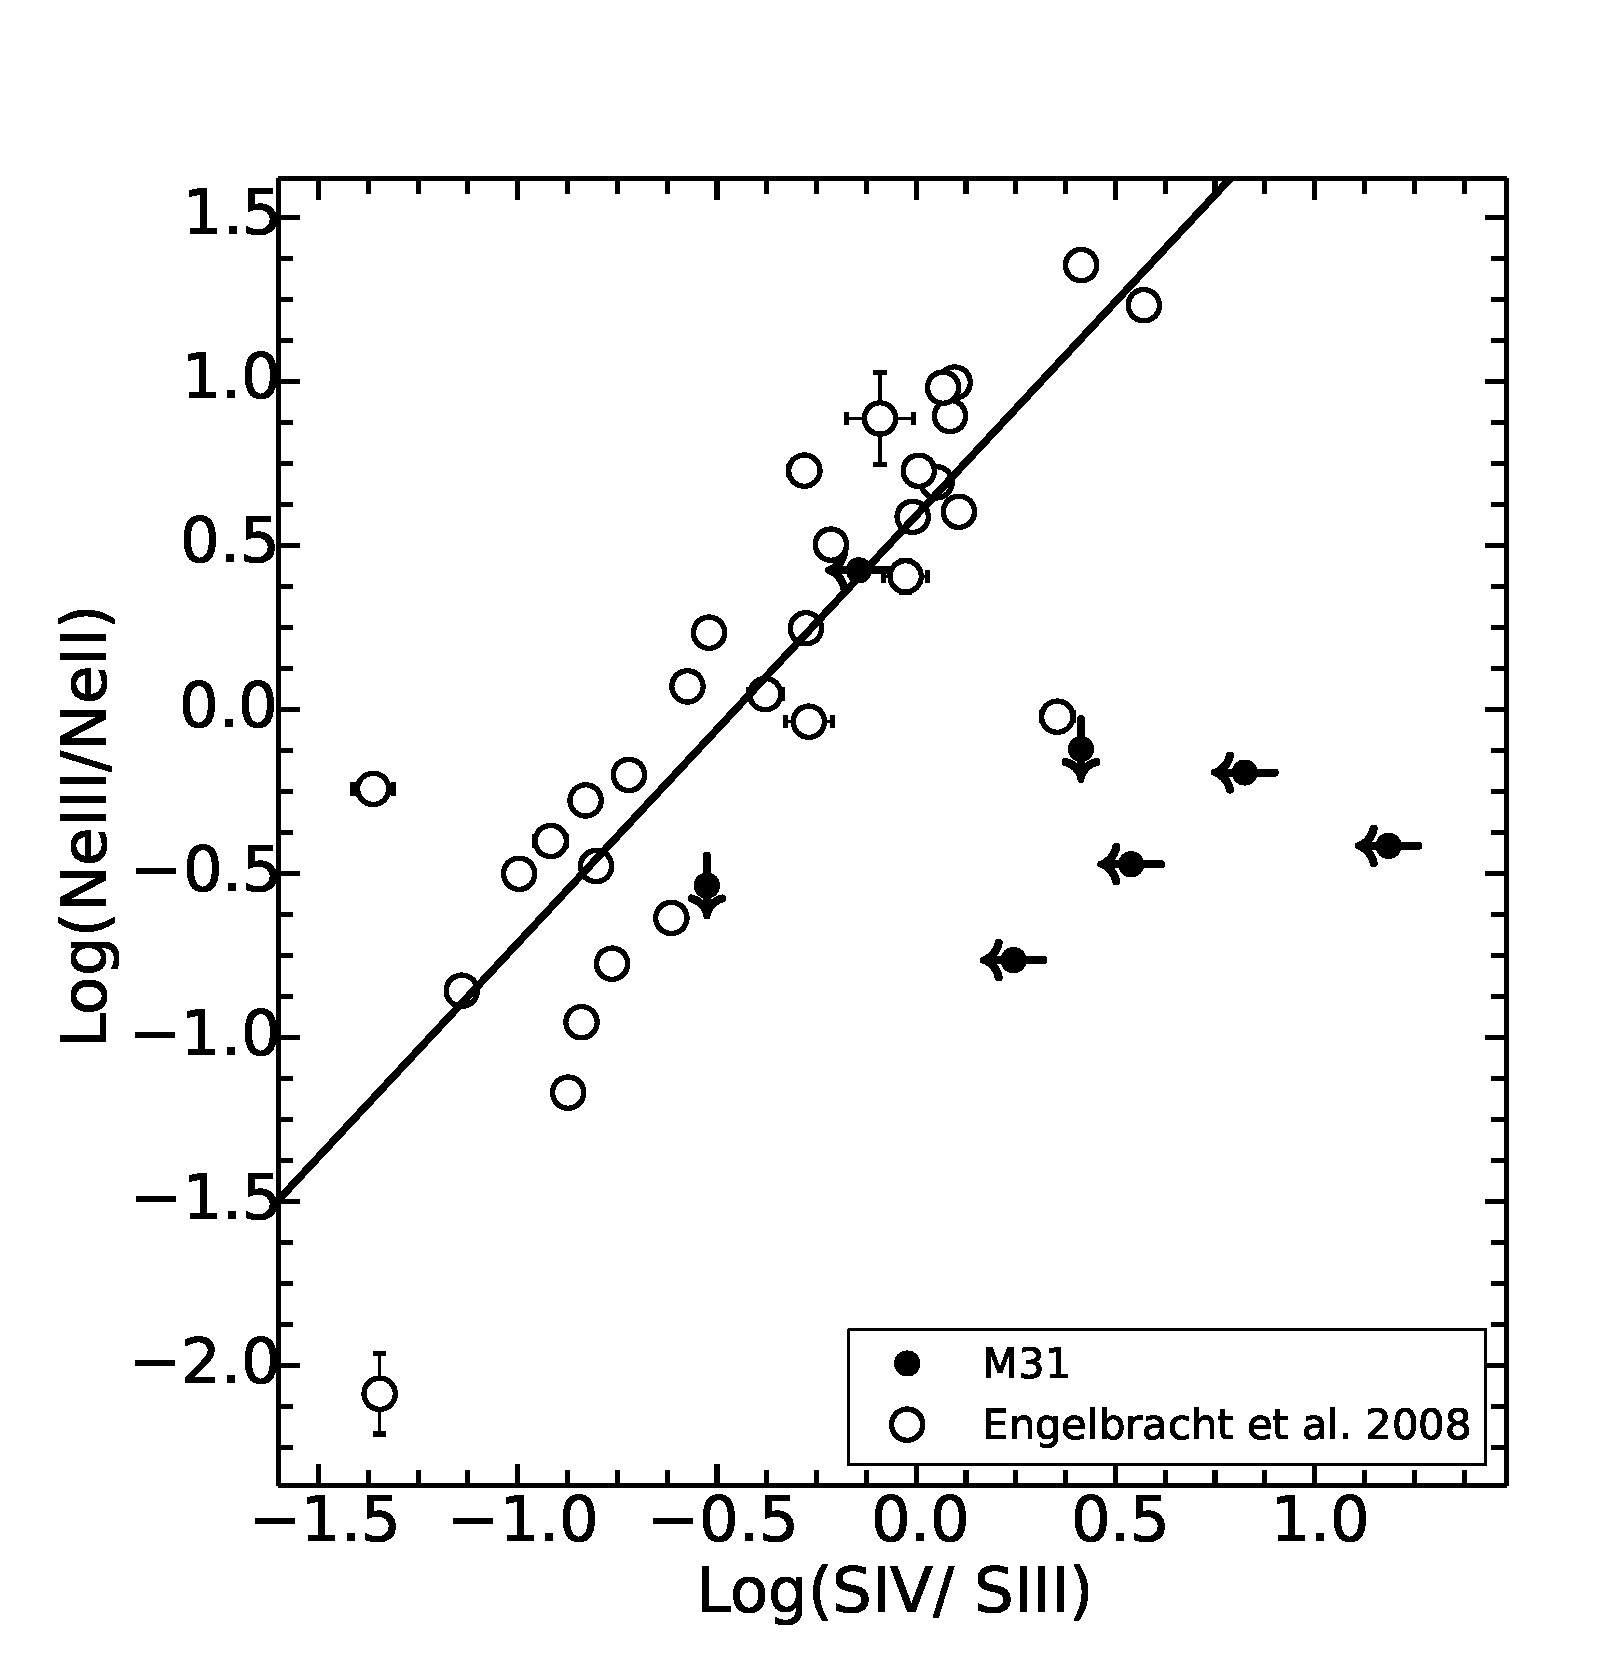
\includegraphics[scale=0.3]{./NevsS.eps}
\caption{ Log([Ne~{\sc iii}]/[Ne~{\sc ii}])  vs Log([S~{\sc iv}]/[S~{\sc iii}]) 18 for the M31 regions in our sample (black dots) and for the starburst sample from Engelbracht (2008; open dots). The straight line is the line of best fit for the starburst sample.}
%\end{center}
\label{SvsNe}
\end{figure}

PAHFIT also returns the emission line strengths and the flux uncertainties of atomic lines. These are listed in Table 4.

	Line ratios of [Ne~{\sc iii}]/[Ne~{\sc ii}] and [S~{\sc iv}]/[S~{\sc iii}] 18 have been used as an indication of the radiation hardness. \citet{Engelbracht_2008} demonstrated that a combination of these two line ratios -which they call the radiation hardness index (RHI)- is a more sensitive indicator of the hardness of the radiation. The RHI values are calculated using
\vspace{5 mm}	
\begin{equation}
{RHI = \left( \log\frac{\textrm{[Ne~{\sc iii}] }}{\textrm{[Ne~{\sc ii}]}} + [0.71 + 1.58\log\frac{\textrm{{[S~{\sc iv}]}}}{\textrm{{[S~{\sc iv}]}}}\right) /2}
\vspace{5 mm}	
\end{equation}

	Here, 1.58 and 0.71 are the slope and the intercept of the [Ne~{\sc iii}]/[Ne~{\sc ii}]  vs [S~{\sc iv}]/[S~{\sc iii}] 18 plot (Figure \ref{SvsNe}) for the starburst sample from \citet{Engelbracht_2008}. The RHI has also been used by \citet{Gordon:2008lr} for M101 observations. To investigate whether the atomic line emission from the selected regions of M31 with the fit parameters described above, we compared them to the starburst sample (Figure \ref{SvsNe}). 
	
	We calculated upper limits for non-detected lines \footnote{To find the upper limits for the flux of missing atomic lines, we assumed the line to be a Gaussian profile with a FWHM as given by PAHFIT. The peak intensity was taken to be 3 times the RMS, where RMS is the root mean square of the noise at the position of a missing line.}. Figure \ref{SvsNe}  shows that the limits are reasonably following the trend for the starburst galaxy sample. Therefore the equation mentioned above was adopted with a simple modification to calculate the RHI values for our sample. For the regions with missing Ne lines, equations 4 was used and for the regions with missing S lines, equation 5 was used. 




\vspace{2 mm}	
\begin{equation}
RHI = \left(0.71 + 1.58\log\frac{\textrm{[S~{\sc iv}]}}{\textrm{[S~{\sc iii}]}}\right)
\vspace{1 mm}	
\end{equation}

\vspace{1 mm}	
\begin{equation}
RHI = \left(\log\frac{\textrm{[Ne~{\sc iii}]}}{\textrm{[Ne~{\sc ii}]}}\right)
\vspace{5 mm}	
\end{equation}
		%\vspace{5 mm}
		
		For Region 2, Region 5 and Region 8 regions, we used the upper limit values of their atomic line intensities to calculated RHI values.
	

